\chapter{Introdução}

  O projeto visa o aumento da qualidade de vida dos alunos a partir do plantio de alimentos dentro do campus, conseguindo, com isso,
  fornecer alimentos saudáveis, para que os estudantes tenham opções de lanches que atendam à essa demanda. Além disso, contribuirá com a
  criação de sombras para espaços de convivência adequados, melhorando o bem-estar dos alunos e reduzindo o estresse com maiores opções de lazer, além de reduzir o calor e aumentar a umidade do ar consideravelmente.

  O projeto se faz viável a partir da contribuição dos alunos e funcionários com a horta. É possível que ela seja utilizada como projeto de extensão para pesquisas e, dependendo do sucesso do projeto, que sirva de exemplo para implatação em outras instituições interessadas, uma vez que o retorno social do projeto é interessante para todos.

\section{Problema}

  Problemas que foram adicionados ao diagrama de fishbone.

  \begin{figure}[!htb]
    \centering
    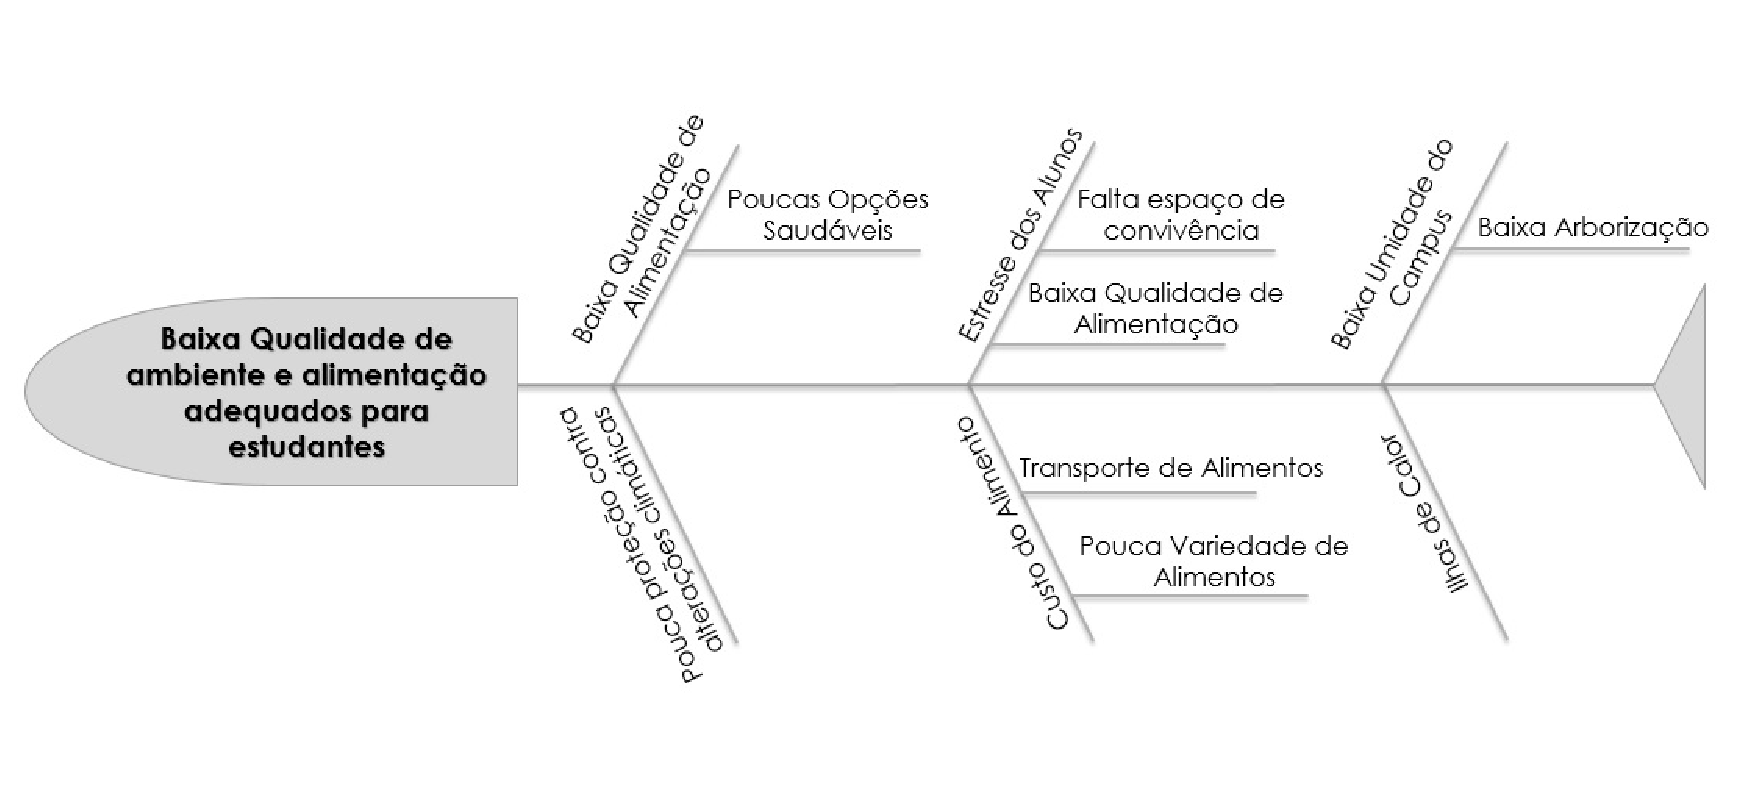
\includegraphics[width=15cm, keepaspectratio=true]{figuras/introducao/fishbone.eps}
    \caption{Diagrama de Fishbone}
  \end{figure}

\subsection{Descrição do problema}

  \newpage

  \begin{table}[!htb]
    \centering
    \begin{tabular}{p{3cm}p{13cm}}
      \toprule
      \textbf{O problema é}                        & O problema dos grandes centros com relação à alimentação se deve ao fato dos altos
                                                     preços dos produtos em comparação com outras localidades, já que são distantes
                                                     da zona rural. O custo com o transporte é alto e, ao chegar nas cidades, os produtos
                                                     chegam no mercado a preços impraticáveis para grande parte da população, prejudicando
                                                     a qualidade da alimentação dos habitantes e fazendo com que recorram a produtos
                                                     industrializados, com custos finais menores, porém pobres em nutrientes.

                                                     Dentro da universidade, os alunos têm grandes problemas em relação alimentação,
                                                     tanto em qualidade quanto em quantidade. A grande maioria só dispõe
                                                     das três refeições diárias ofertadas pelo restaurante universitário e além de os
                                                     alunos não perceberem que os custos de alimentação são altos - pois a maior parte é
                                                     paga pela universidade através dos impostos - existe pouca variedade de alimentos
                                                     fora desse local. É comprovado que estudantes que não se alimentam adequadamente
                                                     possuem baixo desempenho e por isso faz-se necessário que alimentos saudáveis sejam
                                                     mais ofertados para que eles possam comer durante os intervalos.

                                                     Além disso, a falta de arborização dentro do campus prejudica a umidade do ar, e
                                                     aumenta a formação de zonas de calor, que intensificam a sensação térmica local.
                                                     Problemas como estes causam estresse na comunidade acadêmica e prejudicam o
                                                     rendimento de todos no local.                                                                 \\ \midrule
      \textbf{Isto afeta}                          & Comunidade acadêmica                                                                   \\ \midrule
      \textbf{O impacto do problema}               & Prejudica o rendimento acadêmico dos alunos, criação de zonas de calor aumentando a
                                                     sensação térmica, alimentos com poucos nutrientes e com um alto preço.                 \\ \midrule
      \textbf{Uma solução bem sucedida incluiria}  & Plantio de alimentos dentro do campus e a partir desse culitvo conseguir fornecer alimentos
                                                     saudáveis, para que os alunos tenham opções de lanches sem precisar pagar mais por isso.    \\
      \bottomrule
    \end{tabular}
    \caption{Descrição do problema}
  \end{table}

\subsection{Sentença de Posição do Produto}

  \begin{table}[!htb]
    \centering
    \begin{tabular}{p{3cm}p{13cm}}
      \toprule
      \textbf{Para}         & A comunidade acadêmica                                                                                \\ \midrule
      \textbf{Que}          & Necessitam de uma melhor alimentação e bem estar                                                      \\ \midrule
      \textbf{O}            & Projeto Agricultura urbana na FGA                                                                     \\ \midrule
      \textbf{Que é}        & Um projeto social realizado pelos alunos                                                              \\ \midrule
      \textbf{Que oferece}  & Uma alimentação saudável e barata para que os alunos tenham um melhor desempenho acadêmico e uma área
                              que visa o bem estar dos habitantes da FGA, reduzindo o estresse e proporcionando uma opçao saudável de lazer.                       \\
      \bottomrule
    \end{tabular}
    \caption{Sentença de Posição do Produto}
  \end{table}


\section{Metodologia Utilizada}

  A metodologia que iremos utilizar para gerencia a equipe é o framework da metodologia agil SCRUM que é a palavra usada no Rugby para
  descrever uma formação, onde os atletas se reunião para formar estratégias, foi adaptada para a engenharia de software como uma
  metodologia ágil de gerenciamento de projetos.

  \begin{itemize}
    \item Equipes que se auto-organizam;
    \item É um framework da metodologia ágil para organizar e gerenciar projetos;
    \item Projetos Scrum progridem em uma série de sprints (conjunto de tarefas);
    \item Scrum encara a mudança como parte natural do processo de desenvolvimento.
  \end{itemize}

\subsection{Papeis}

  \begin{description}
    \item[Scrum Master ou Gerente de Projeto] \

      Na metodologia ágil SCRUM o scrum master não é considerado um gerente, pois a boas práticas da metodologia que diz que a equipe
      tem que se auto-gerenciar sendo que os gerentes ou scrum master no nosso projeto serão responsáveis apenas para:

      \begin{itemize}
        \item Aplicação dos valores e práticas do Scrum;
        \item Garante a plena funcionalidade e produtividade da equipe;
        \item Garante a colaboração entre os diversos papéis e funções;
        \item Faz parte diretamente da equipe tendo que trabalhar também;
        \item No nosso caso será a gerente do projeto e o subgerente de logística.
      \end{itemize}

    \item[Product Owner ou Subgerentes do Projeto] \

      Na metodologia ágil SCRUM o product owner é considerado o stakeholder que irá fazer parte da equipe, porém como um dos stakeholder
      são os próprios alunos, os product owner serão os subgerentes de cada equipe do projeto e a gerente do projeto, que terá como
      responsabilidade:

      \begin{itemize}
        \item Entra em contato direto com os stakeholders e com a equipe;
        \item Marca reuniões com os stakeholders e com a equipe;
        \item Responsável por definir manutenção e mudança dos requisitos;
        \item No nosso caso será os subgerentes de cada equipe e a gerente de pesquisa e desenvolvimento do projeto;
        \item Faz parte diretamente da equipe, tendo que trabalho como qualquer membro.
      \end{itemize}

    \item[Equipe de Projeto] \

      A equipe de projeto inclui todos os demais membros da equipe e inclui também o scrum master e os product owners, e são responsaveis
      por:

      \begin{itemize}
        \item Realiza o trabalho técnico do projeto, pesquisa e desenvolvimento;
        \item Todos fazem parte da equipe, logo todos trabalham;
        \item Multifuncional (5 engenharias);
        \item Auto-Organizado (Todos trabalham sem precisar de ficar mandando);
        \item Auto-Gerenciado (todos devem ter noção do que tem que fazer).
      \end{itemize}

  \end{description}

\subsection{Artefatos}

  Os artefatos da metodologia ágil SCRUM são mais voltada a organização e gerenciamento de tarefas na qual não precisa para esse projeto
  ser documentado, só será usado na ferramenta trello para melhor organização do andamento do projeto:

  \begin{description}
    \item[Product Backlog] \
      \begin{itemize}
        \item Lista com todas a tarefas que iremos realizar no projeto, faz parte do kanban;
        \item Priorizado pelo scrum master e o product owner;
        \item Re-priorizado no início de cada Sprint.
      \end{itemize}
    \item[Sprint Backlog] \
      \begin{itemize}
        \item Sprint é um conjunto de tarefas que será realizada em 1 semana de trabalho;
        \item Cada sprint deve ter um objetivo bem claro do que fazer na semana;
        \item Definido a partir da lista do Product Backlog;
        \item Cada indivíduo escolhe o tarefa que fará. Trabalhos nunca são atribuídos, só em casos extremos como atraso do projeto ou
          falta de comprometimento dos membros;
        \item Qualquer membro da equipe pode adicionar, apagar ou mudar tarefas desde que haja o consentimento da equipe toda,
          principalmente do product owner e do scrum master.
      \end{itemize}
  \end{description}

\subsection{Eventos}

  Os eventos serão baseados no scrum que é um framework da metodologia ágil para melhor gerenciamento e organização do projeto, os
  eventos são:

  \begin{description}
    \item[Planejamento da Sprint] \
      \begin{itemize}
        \item Todo o planejamento da sprint será realizado na ferramenta trello utilizando a estratégia de kanban;
        \item Basicamente é a reunião semanal que faremos para definir as tarefas da semana, ocorreram nas segundas na hora da aula,
          onde cada subgerente ou product owner ficará responsavel em definir tarefas para sua equipe;
        \item A equipe seleciona itens do Product Backlog com quais compromete-se, dentro do kanban (A fazer);
        \item O Sprint Backlog é criado (tarefas da semana);
        \item As tarefas são identificadas e estimadas (em nível de dificuldade e quais e quantos membros irão faze-lo de acordo com o
          nível de dificuldade);
        \item Todo trabalho de planejamento é feito de forma colaborativa, ou seja, todos participam;
        \item É feito um planejamento de alto nível (sem enrolação, direto ao foco).
      \end{itemize}
    \item[Stand-up] \

      Apesar de que no SCRUM o stand-up é realizado de forma presencial e todo de pé como o nome sugere, no nosso projeto iremos fazer
      de forma online, na ferramenta do telegram, e não precisa ficar de pé.

      \begin{itemize}
        \item Ocorrerar em cada equipe, e será organizada pelos subgerentes ou product owner para saber o que cada integrante está
          fazendo e quais dificuldades esta enfrentando;
        \item Duração máxima de 15min todo dia caso for preciso;
        \item Não se procura solução de problemas durante a reunião;
        \item Cada um falará o que já fez da tarefa e o que falta fazer, e falará as dificuldades que está tendo e qual solução irá
          tomar em relação a isso.
      \end{itemize}

    \item[Revisão e Retrospectiva da Sprint] \
      \begin{itemize}
        \item Feita após cada Sprint;
        \item Equipe apresenta os resultados obtidos durante o Sprint no documento especificado no google driver, será realizado nas
          segundas durante a aula e os subgerentes começam o trabalho de passar tudo para o LaTeX de forma organizada;
        \item Na reunião a equipe discute o que gostaria de iniciar a fazer, parar de fazer e continuar fazendo;
        \item A equipe inteira irá organizar os arquivo para passar para o LaTeX de modo que não sobrecarregue quem irá passar
          todo o conteúdo.
      \end{itemize}
  \end{description}

\section{Objetivos do projeto}

  O projeto da Agricultura Urbana na FGA pretende implementar a produção de alimentos dentro do campus da UnB $-$ Gama, de modo a
  aproveitar os espaços ociosos disponíveis, respeitando a vegetação nativa e o projeto do campus, criando locais de convivência para
  os alunos. Além disso o projeto vai permitir que estudantes de outros campis possam realizar projetos de extensão com estudos sobre
  a automação, os métodos de plantio e o tratamento do solo utilizados nesse projeto.

  O projeto vai abranger vários métodos de plantio com a ocupação da parede lateral do UAC (unidade acadêmica), revitalização da
  área entre os prédios do UAC e o restaurante universitário (RU), com plantação de árvores para criação de sombras para espaço de
  lazer, gerando também alimentos, dos quais os alunos poderão acompanhar o processo desde o plantio até a colheita,
  gratuitamente e no momento que quiser. Além disso, o plano diretor do campus inclui “teto verde”, ou seja, a estrutura está
  preparada para receber plantações na laje, de forma a propiciar a criação de uma horta verde organica.

  Dessa forma os alunos poderão fazer uso dos produtos do plantio dentro da universidade por ser um projeto aberto, com apoio da
  comunidade acadêmica, totalmente gratuito, uma vez que o retorno social é maior que a relev\^{a}ncia econ\^{o}mica e uma das premissas
  do nosso trabalho conta com financiamento da universidade para trazer benefícios aos alunos, servidores, técnicos e terceirizados da FGA.

\section{Benefícios}

  Normalmente hortas de verduras, legumes e temperos frescos colhidos na hora garantem maior qualidade de nutrientes, além de livrar o
  consumidor dos agrotóxicos e fertilizantes, favorece a redução do consumo de sal, respeita a natureza, tem um custo aceitável e
  favorece o desempenho dos alunos.

  Dessa forma, de modo geral, temos diversos benefícios, como: aumento da qualidade de vida dos alunos, melhoraria na qualidade da alimentação, criação de sombras para o bem estar dos estudantes, diminuição do calor, possível utilização para projetos de extensão, uso dos produtos do plantio dentro da universidade, retorno social e redução dos custos alimentícios.

\section{Premissas}

  As principais premissas são: retorno social, pesquisa e extensão, inalteração do projeto da faculdade e autorização da direção da faculdade.

\section{Restrições}

  As principais retrições encontradas foram: legislação ambiental, plano diretor, legislação interna e patrim\^{o}nio público.

\section{Requisitos}

  As técnicas de elicitação que serão utilizadas para adquirir possíveis requisitos e, até mesmo, para analisar os existentes será
  entrevistas e brainstormings.

  Os requisitos determinados e coletados de antemão para o projeto são:

  \begin{itemize}
    \item \textbf{R01}: O projeto deve ter uma estrutura e materiais adequados de boa qualidade para a execução do projeto;
    \item \textbf{R02}: O projeto deve engoblar os alimentos mais adequados para o plantio com valor nutricional considerável, de acordo com o clima e entre outros desafios presentes na faculdade;
    \item \textbf{R03}: O projeto de ter sensores automatizados para acompanhamento da produção;
    \item \textbf{R04}: O projeto deve ter um gerenciamento constante do sistema, podendo ser de forma manual ou automática;
    \item \textbf{R05}: O projeto deve aproveitar rejeitos, adubos e etc, e deve ter uma geração de energia eficiente;
    \item \textbf{R06}: O projeto deve ser irrigado de forma automatizada e econ\^{o}mica, talvez com alguma fonte de água reutilizável.
  \end{itemize}

\section{Canvas}

  O canvas de projeto se encontra no anexo \ref{canvas}.

